\documentclass[11pt,twocolumn,oneside,openany,headings=optiontotoc,11pt,numbers=noenddot]{article}

\usepackage[a4paper]{geometry}
\usepackage[utf8]{inputenc}
\usepackage[T1]{fontenc}
\usepackage{lmodern}
\usepackage[ngerman]{babel}
\usepackage{ngerman}

\usepackage[onehalfspacing]{setspace}

\usepackage{fancyhdr}
\usepackage{fancybox}

\usepackage{rotating}
\usepackage{varwidth}

%Struktogramme
\usepackage[german,curves]{struktex}

\usepackage{pdflscape}
\usepackage{changepage}
\usepackage{graphicx}
\usepackage[bottom]{footmisc}
\usepackage{transparent}
\usepackage{graphbox}
\graphicspath{
	{Pics/PDFs/}
	{Pics/JPGs/}
	{Pics/PNGs/}
}
\usepackage{caption}
\usepackage{wrapfig}
\usepackage{marginnote}
\usepackage{tabularx}
\usepackage{dashrule}
\usepackage{soulutf8}
\usepackage{hhline}
%arydshln suppresses vertical lines in table
%\usepackage{arydshln}
\usepackage{multirow}
\usepackage{enumerate}
\usepackage[hidelinks]{hyperref}
\usepackage{listings}

\usepackage[table]{xcolor}
\usepackage{array}
\usepackage{enumitem,amssymb,amsmath}
\usepackage{interval}
\usepackage{cancel}
\usepackage{stmaryrd}
\usepackage{wasysym}
\usepackage{polynom}
\usepackage{diagbox}
\usepackage{dashrule}
\usepackage{framed}
\usepackage{mdframed}
\usepackage{karnaugh-map}
\usepackage{pdfpages}

\usepackage{blindtext}

\usepackage{eso-pic}

\usepackage{amssymb}
\usepackage{eurosym}

\usepackage[pages=some]{background}
\pagestyle{headings}
\renewcommand{\headrulewidth}{0.2pt}
\renewcommand{\footrulewidth}{0.2pt}
\newcommand*{\underdownarrow}[2]{\ensuremath{\underset{\overset{\Big\downarrow}{#2}}{#1}}}
\setlength{\fboxsep}{5pt}
\newcommand{\explainBelow}[3]{\underbrace{#1}_{\parbox{\widthof{#3}}{\footnotesize\raggedright #2}}}
\newcommand{\explainAbove}[3]{\overbrace{#1}^{\parbox{\widthof{#3}}{\footnotesize\raggedright #2}}}
\newcommand\footnoteref[1]{\protected@xdef\@thefnmark{\ref{#1}}\@footnotemark}


% Codestyle defined
\definecolor{codegreen}{rgb}{0,0.6,0}
\definecolor{codegray}{rgb}{0.5,0.5,0.5}
\definecolor{codepurple}{rgb}{0.58,0,0.82}
\definecolor{backcolour}{rgb}{0.95,0.95,0.92}
\definecolor{deepgreen}{rgb}{0,0.5,0}
\definecolor{darkblue}{rgb}{0,0,0.65}
\definecolor{mauve}{rgb}{0.40, 0.19,0.28}
\colorlet{exceptioncolour}{yellow!50!red}
\colorlet{commandcolour}{blue!60!black}
\colorlet{numpycolour}{blue!60!green}
\colorlet{specmethodcolour}{violet}

%Neue Spaltendefinition
\newcolumntype{L}[1]{>{\raggedright\let\newline\\\arraybackslash\hspace{0pt}}m{#1}}
\newcolumntype{M}{>{\centering\arraybackslash}X}
\newcommand{\cmnt}[1]{\ignorespaces}
%Textausrichtung ändern
\newcommand\tabrotate[1]{\rotatebox{90}{\raggedright#1\hspace{\tabcolsep}}}

%Intervall-Konfig
\intervalconfig {
	soft open fences
}

%Bash
\lstdefinestyle{BashInputStyle}{
	language=bash,
	basicstyle=\small\sffamily,
	backgroundcolor=\color{backcolour},
	columns=fullflexible,
	backgroundcolor=\color{backcolour},
	breaklines=true,
}
%Java
\lstdefinestyle{JavaInputStyle}{
	language=Java,
	backgroundcolor=\color{backcolour},
	aboveskip=1mm,
	belowskip=1mm,
	showstringspaces=false,
	columns=flexible,
	basicstyle={\footnotesize\ttfamily},
	numberstyle={\tiny},
	numbers=none,
	keywordstyle=\color{purple},,
	commentstyle=\color{deepgreen},
	stringstyle=\color{blue},
	emph={out},
	emphstyle=\color{darkblue},
	emph={[2]rand},
	emphstyle=[2]\color{specmethodcolour},
	breaklines=true,
	breakatwhitespace=true,
	tabsize=2,
}
%Python
\lstdefinestyle{PythonInputStyle}{
	language=Python,
	alsoletter={1234567890},
	aboveskip=1ex,
	basicstyle=\footnotesize,
	breaklines=true,
	breakatwhitespace= true,
	backgroundcolor=\color{backcolour},
	commentstyle=\color{red},
	otherkeywords={\ , \}, \{, \&,\|},
	emph={and,break,class,continue,def,yield,del,elif,else,%
		except,exec,finally,for,from,global,if,import,in,%
		lambda,not,or,pass,print,raise,return,try,while,assert},
	emphstyle=\color{exceptioncolour},
	emph={[2]True,False,None,min},
	emphstyle=[2]\color{specmethodcolour},
	emph={[3]object,type,isinstance,copy,deepcopy,zip,enumerate,reversed,list,len,dict,tuple,xrange,append,execfile,real,imag,reduce,str,repr},
	emphstyle=[3]\color{commandcolour},
	emph={[4]ode, fsolve, sqrt, exp, sin, cos, arccos, pi,  array, norm, solve, dot, arange, , isscalar, max, sum, flatten, shape, reshape, find, any, all, abs, plot, linspace, legend, quad, polyval,polyfit, hstack, concatenate,vstack,column_stack,empty,zeros,ones,rand,vander,grid,pcolor,eig,eigs,eigvals,svd,qr,tan,det,logspace,roll,mean,cumsum,cumprod,diff,vectorize,lstsq,cla,eye,xlabel,ylabel,squeeze},
	emphstyle=[4]\color{numpycolour},
	emph={[5]__init__,__add__,__mul__,__div__,__sub__,__call__,__getitem__,__setitem__,__eq__,__ne__,__nonzero__,__rmul__,__radd__,__repr__,__str__,__get__,__truediv__,__pow__,__name__,__future__,__all__},
	emphstyle=[5]\color{specmethodcolour},
	emph={[6]assert,range,yield},
	emphstyle=[6]\color{specmethodcolour}\bfseries,
	emph={[7]Exception,NameError,IndexError,SyntaxError,TypeError,ValueError,OverflowError,ZeroDivisionError,KeyboardInterrupt},
	emphstyle=[7]\color{specmethodcolour}\bfseries,
	emph={[8]taster,send,sendMail,capture,check,noMsg,go,move,switch,humTem,ventilate,buzz},
	emphstyle=[8]\color{blue},
	keywordstyle=\color{blue}\bfseries,
	rulecolor=\color{black!40},
	showstringspaces=false,
	stringstyle=\color{deepgreen}
}

\lstset{literate=%
	{Ö}{{\"O}}1
	{Ä}{{\"A}}1
	{Ü}{{\"U}}1
	{ß}{{\ss}}1
	{ü}{{\"u}}1
	{ä}{{\"a}}1
	{ö}{{\"o}}1
}

% Neue Klassenarbeits-Umgebung
\newenvironment{worksheet}[3]
% Begin-Bereich
{
	\newpage
	\sffamily
	\setcounter{page}{1}
	\ClearShipoutPicture
	\AddToShipoutPicture{
		\put(55,761){{
				\mbox{\parbox{385\unitlength}{\tiny \color{codegray}BBS I Mainz, #1 \newline #2
						\newline #3
					}
				}
			}
		}
		\put(455,761){{
				\mbox{\hspace{0.3cm}
\includegraphics[width=0.2\textwidth]{../../logo.pdf}}
			}
		}
	}
}
% End-Bereich
{
	\clearpage
	\ClearShipoutPicture
}

\setlength{\columnsep}{3em}
\setlength{\columnseprule}{0.5pt}

\geometry{left=1.50cm,right=2.00cm,top=3.00cm,bottom=1.00cm,includeheadfoot}
\pagenumbering{arabic}
\pagestyle{plain}

\begin{document}
	\begin{worksheet}{BS FI 1. Lehrjahr}{LF 4 - Einfache IT-Systeme}{Digitaltechnik - Zahlensysteme - Rechnen mit Binärzahlen}
		\setcounter{section}{2}
		\setcounter{page}{7}
		\section{Rechnen mit Binärzahlen}
		In der Mathematik können wir beliebig große Zahlen darstellen. Innerhalb eines Computers ist der Speicherplatz aber beschränkt und somit auch die Anzahl der möglichen Stellen einer Binärzahl.\\
		Betrachten wir folgendes Beispiel:\\
		\par\noindent
		\begin{tabularx}{0.48\textwidth}{|M|M|M|}
			\# Bit & Dez & Bin\\
			\hline
			\multirow{8}{*}{3} & 0 & 000\\
			\cline{2-3}
			& 1 & 001\\
			\cline{2-3}
			& 2 & 010\\
			\cline{2-3}
			& 3 & 011\\
			\cline{2-3}
			& 4 & 100\\
			\cline{2-3}
			& 5 & 101\\
			\cline{2-3}
			& 6 & 110\\
			\cline{2-3}
			& 7 & 111\\
			\hline
		\end{tabularx}\\
		\par\noindent
		Bei drei zur Verfügung stehenden Bits lassen sich also insgesamt nur acht verschiedene Zahlen (0-7) darstellen.
		\subsection{Wie werden Binärzahlen addiert?}
		In einem Stellenwertsystem, unabhängig von der Basis, können wir addieren, wie wir es aus der Grundschule kennen.\\
		Dabei dürfen wir aber lediglich die zur Verfügung stehenden Ziffern verwenden.\\
		\tiny{Im \textit{Oktal} können wir nur die Ziffern \(0 - 7\) verwenden.}\normalsize\\
		Für das Binärsystem ergeben sich somit folgende Regeln:\\
		\par\noindent
		\begin{tabularx}{0.48\textwidth}{ccccc}
			0 & + & 0 & = & 0\\
			0 & + & 1 & = & 1\\
			1 & + & 0 & = & 1\\
			1 & + & 1 & = & 0
		\end{tabularx}\\
		\par\noindent
		Man mag sich fragen, was ist da bei \(1 + 1 = 0\) passiert?\\
		Wie auch im Dezimalsystem kommt es zu einem \textbf{Übertrag}, wenn unsere Summe den Wert der \textit{Basis} des Stellenwertsystems annimmt.\\
		\begin{framed}
			\noindent
			Wir betrachten das folgende Beispiel:\\
			\par\noindent
			\textbf{Dezimal}: \(7 + 11 = 18\)\\
			\textbf{Binär}: \( 111 + 1011 = 10010\)\\
			\par\noindent
			Wie kommen wir darauf:\\
			\par\noindent
			\begin{tabularx}{0.4\textwidth}{llllll}
				& & 0 & 1 & 1 & 1\\
				+ & & 1 & 0 & 1 & 1\\
				\\
				\tiny{\color{codegray}{Übertrag}} & \color{codegray}{1} & \color{codegray}{1} & \color{codegray}{1} & \color{codegray}{1} & \\
				\cline{1-6}
				\\
				& 1 & 0 & 0 & 1 & 0\\
				\cline{2-6}
			\end{tabularx}
		\end{framed}
		\noindent
		Was fällt bezüglich der Anzahl der Stellen der beiden Summanden und der Summe auf?\\
		\par\noindent
		Die Regeln der Addition lassen sich wie folgt festhalten:\\
		\par\noindent
		\begin{tabularx}{0.48\textwidth}{MM|MM}
			\(x_1\) & \(x_2\) & E & O\\
			\hline
			0 & 0 & 0 & 0\\
			0 & 1 & 1 & 0\\
			1 & 0 & 1 & 0\\
			1 & 1 & 0 & 1\\
		\end{tabularx}\\
		\par\bigskip\noindent
		Wir haben nun die Addition von Binärzahlen kennengelernt und können diese ziemlich souverän anwenden.\\
		Was wir aber noch nicht können, ist die Subtraktion. Der Computer selbst ist auch nicht in der Lage zu subtrahieren. Was intern passiert, wenn \(3 - 2\) gerechnet wird, ist \(3 + (-2)\). Der Computer addiert also die \(-2\) zur \(3\) hinzu. Um das genauer zu verstehen, schauen wir uns die Negativdarstellung von Binärzahlen an.
		\subsection{Darstellung negativer Zahlen}
		\textit{\textbf{Ausgangsproblem:} Wie stellt man eine negative Zahl im Binärsystem dar? z.B.: \(-5\)}\\
		\subsubsection{Negative Zahlen}
		Im Allgemeinen haben wir für die Darstellung einer Zahl \(n\) Bit zur Verfügung. Das heißt, haben wir 3 Bit, so können wir die Zahlen von \(0 - 7 (2^3-1)\) darstellen.\\
		Um nun aber positive und negative Zahlen darstellen zu können, reservieren wir das vorderste (\textbf{M}ost \textbf{S}ignificant \textbf{B}it) Bit als Vorzeichen. Hier gilt die Zuordnung:\\
		\(MSB = 0 \Rightarrow\) Zahl ist positiv.\\
		\(MSB = 1 \Rightarrow\) Zahl ist negativ.\\
		\par\noindent
		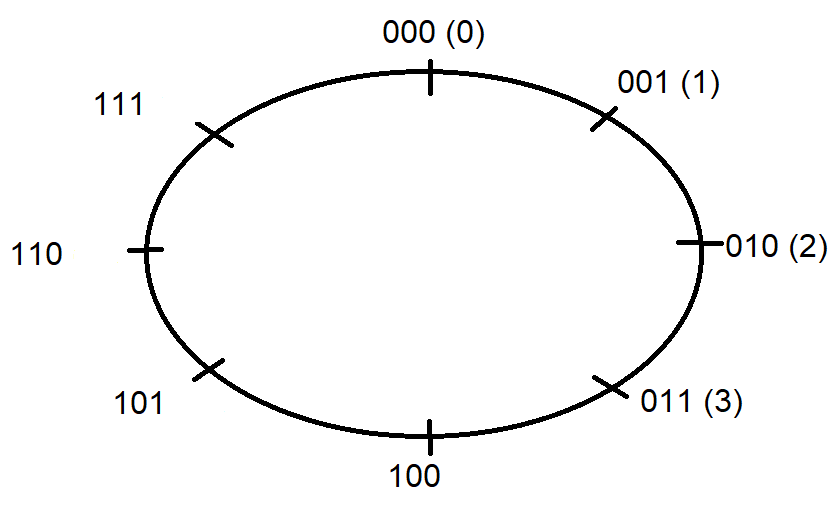
\includegraphics[width=0.48\textwidth]{../99_Bilder/negZahlenkreisoZahlen.png}\\
		\par\noindent
		Bleibt herauszufinden, welche Zahlen mit der \(1\ldots\) Darstellung gegeben sind.\\
		Hierfür betrachten wir Beispielhaft eine der vier Zahlen.\\
		\textbf{\underline{Beispiel:}} Welche Zahl müssen wir addieren, um wieder zur Null (0) zu gelangen:\\
		\begin{tabularx}{0.48\textwidth}{rc|llll}
			 & ? & & 1 & 0 & 1\\
			 + & 3 & & 0 & 1 & 1\\
			 \cline{1-6}
			 & 0 & (1) & 0 & 0 & 0
		\end{tabularx}
		Auf die gleiche Weise können wir herausfinden, welche Zahlen die anderen \(1\dots\) Darstellen repräsentieren.\\
		\par\noindent
		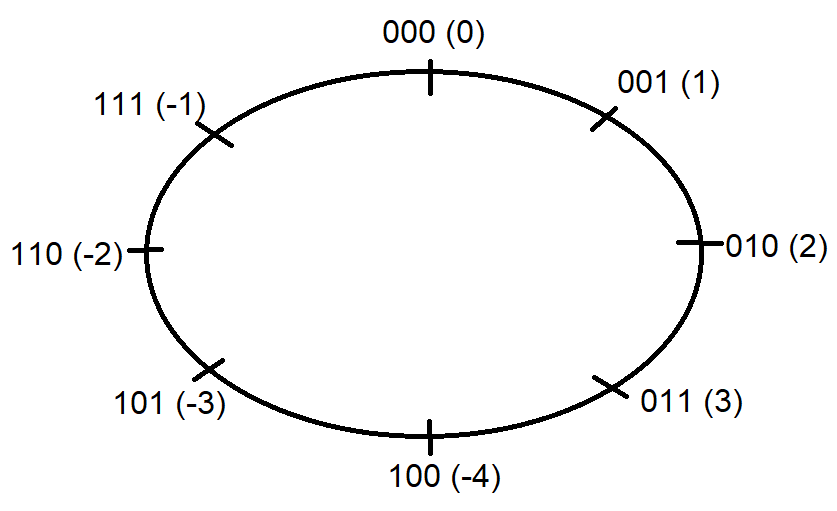
\includegraphics[width=0.48\textwidth]{../99_Bilder/negZahlenkreis.png}\\
		\par\noindent
		\textit{Bleibt zu klären, wie man die Negativdarstellung erhält, ohne jedes Mal zu zeichnen oder auszuprobieren.}\\
		Hierfür müssen wir zwei Schritte ausführen, welche nachfolgend kurz erklärt werden.
		\subsubsection{Einerkomplement}
		Wie eben bereits erwähnt, müssen die Zahl und ihre negative Zahl zusammen Null (0) ergeben. Zunächst bestimmen wir also die Binärzahl, so dass wir bei der größten mit \(n\) Bit darstellbaren Zahl sind.\\
		\tiny{Im Fall von 3 Bit ist das \(111_2\), bei 4 Bit dann \(1111_2\).}\normalsize\\
		Diese ominöse Zahl erhält man, indem man \textbf{alle Bit invertiert} (also umdreht). Diese Darstellung nennt man auch \textbf{Einerkomplement}.\\
		\textbf{\underline{Beispiel:}} \(101_2 \Rightarrow 010_2\).\\
		\par\noindent
		\begin{tabularx}{0.48\textwidth}{c|lll||rrr|c}
			\multicolumn{4}{c||}{Zahldarstellung} & \multicolumn{4}{c}{Einerkomplement}\\
			Dez & \multicolumn{3}{c||}{Bin} & \multicolumn{3}{c}{Bin} & Dez\\
			\cline{1-8}
			0 & 0 & 0 & 0 & 1 & 1 & 1 & 7\\
			1 & 0 & 0 & 1 & 1 & 1 & 0 & 6\\
			2 & 0 & 1 & 0 & 1 & 0 & 1 & 5\\
			3 & 0 & 1 & 1 & 1 & 0 & 0 & 4\\
			4 & 1 & 0 & 0 & 0 & 1 & 1 & 3\\
			5 & 1 & 0 & 1 & 0 & 1 & 0 & 2\\
			6 & 1 & 1 & 0 & 0 & 0 & 1 & 1\\
			7 & 1 & 1 & 1 & 0 & 0 & 0 & 0
		\end{tabularx}\\
		\subsubsection{Zweierkomplement}
		In der Tabelle ist erkennbar, eine Zahl und ihre Gegenkomponente ergeben die größte mit \(n\) Bit darstellbare Zahl. Um nun alle \(n\) auf Null (0) zu bringen und einen Übertrag an der höchsten Stelle zu erhalten, also aus dem darstellbaren Zahlenbereich raus zu fallen, müssen wir \(1\) addieren.\\\par\noindent
		\textbf{\underline{Beispiel:}} Wir haben 3 Bit und möchten das Zweierkomplement von \(2\).\\
		\par\noindent
		\begin{tabularx}{0.48\textwidth}{l|cccl}
			2 & 0 & 1 & 0 & \textit{\small{Zahl}}\\
			\cline{1-5}
			\\
			& 1 & 0 & 1 & \textit{\small{Einerkomplement}}\normalsize\\
			+ & & & 1 & \textit{\small{Addiere 1}}\normalsize\\
			& & \color{codegray}{\tiny{1}} & & \textit{\tiny{Übertrag}}\\
			\cline{1-5}\normalcolor\normalsize
			& 1 & 1 & 0 & \textit{\small{Zweierkomplement}}\normalsize
		\end{tabularx}\\
		\par\noindent
		\rule{0.48\textwidth}{0.1pt}\\
		Es gilt also folgendes:\\
		Für das \textbf{Zweierkomplement} invertieren wir alle Bit (\textit{Einerkomplement}) und \textit{addieren dann 1}.\\
		\par\noindent
		Möchten wir die \textbf{Negativdarstellung einer Zahl}, so stellen wir die Zahl zunächst auf bekannte Weise binär dar. Im Anschluss bilden wir das Zweierkomplement.\\
		\par\noindent
		Beinhaltet die \textbf{Zahldarstellung ein VZ} (ist in der Regel angegeben), so entscheidet diese VZ über unser weiteres Vorgehen.\\
		Wenn \(\mathbf{VZ = 0}\), dann ist die dargestellte Zahl positiv. Wir bestimmen also \textit{aus der Zahldarstellung die Dezimalzahl}.\\
		Ist \(\mathbf{VZ = 1}\), handelt es sich um eine negative Zahl. Wir bilden also das \textit{Zweierkomplement und bestimmen anschließend die Dezimaldarstellung}.\\
		\par\noindent
		\textbf{\underline{Beispiel:}}\\
		Bilden Sie das Zweierkomplement von \(100110_2\)\\
		\begin{tabularx}{0.48\textwidth}{rllllll|l}
			& 0 & 1 & 1 & 0 & 0 & 1 & \textit{Einerkomplement}\\
			+ & & & & & & 1 & \textit{Addiere 1}\\
			& & & & &  \color{codegray}{\tiny{1}} & & \textit{\tiny{Übertrag}}\normalsize\\
			\cline{1-8}
			& 0 & 1 & 1 & 0 & 1 & 0 & \textit{Zweierkomplement}
		\end{tabularx}\\
		\par\noindent
		\rule{0.48\textwidth}{0.1pt}\\
		\par\noindent
		Stellen Sie \(\mathbf{-9_{10}}\) mit 5 Bit dar.\\
		Bestimme zunächst die Dezimaldarstellung von 9 mit 5 Bit \(\Rightarrow 01001_2\)\\
		\par\noindent
		\begin{tabularx}{0.48\textwidth}{rlllll|l}
			& 1 & 0 & 1 & 1 & 0 & \textit{Einerkomplement}\\
			+ & & & & & 1 & \textit{Addiere 1}\\
			& & & & & & \textit{\tiny{Übertrag}}\normalsize\\
			\cline{1-7}
			& 1 & 0 & 1 & 1 & 1 & \textit{Zweierkomplement}
		\end{tabularx}\\
		\par\noindent
		Damit folgt: \(-9_{10} = 10111_{2}\)\\
		\par\noindent
		\rule{0.48\textwidth}{0.1pt}\\
		\par\noindent
		Geben Sie zu folgender Darstellung \textbf{mit} Vorzeichenbit an, um welche Zahl es sich handelt.\\
		\colorbox{green!10}{\(1\)}\(00110_{2}\): \(VZ = 1 \Rightarrow \) negative Zahl.\\
		\par\noindent
		\begin{tabularx}{0.48\textwidth}{rllllll|l}
			& 0 & 1 & 1 & 0 & 0 & 1 & \textit{Einerkomplement}\\
			+ & & & & & & 1 & \textit{Addiere 1}\\
			& & & & & \color{codegray}{\tiny{1}} & & \textit{\tiny{Übertrag}}\normalsize\\
			\cline{1-8}
			& 0 & 1 & 1 & 0 & 1 & 0 & \textit{Zweierkomplement}\\
			& & 16 & 8 &  & 2 & & = 26
		\end{tabularx}\\
		\par\noindent
		Damit folgt: \(101101_2 = -26_{10}\)\\
		\par\noindent
		\rule{0.48\textwidth}{0.1pt}\\
		\par\noindent
		Geben Sie zu folgender Darstellung \textbf{mit} Vorzeichenbit an, um welche Zahl es sich handelt.\\
		\colorbox{green!10}{\(0\)}\(01101_{2}\): \(VZ = 0 \Rightarrow \) positive Zahl.\\
		\par\noindent
		\begin{tabularx}{0.48\textwidth}{llllllr}
			0 & 0 & 1 & 1 & 0 & 1\\
			& & 8 & 4 & & 1 & = 13
		\end{tabularx}\\
		\par\noindent
		Damit folgt: \(001101_2 = 13_{10}\)\\
		\subsection{Wertebereich}
		Durch die Reservierung des MSB als Vorzeichenbit (VZ), bleiben uns nur noch 2 Bit für die Zahldarstellung. Wir können also \textbf{im positiven} von \(0 - 3 (2^2-1)\) und \textbf{im negativen} von \(-1 - (-4) (2^2)\).\\
		\par\noindent
		\begin{tabularx}{0.48\textwidth}{c|lll||rrr|c}
			\multicolumn{4}{c||}{Zahldarstellung} & \multicolumn{4}{c}{Zweierkomplement}\\
			Dez & \multicolumn{3}{c||}{Bin} & \multicolumn{3}{c}{Bin} & Dez\\
			\cline{1-8}
			0 & 0 & 0 & 0 & 0 & 0 & 0 & 0\\
			1 & 0 & 0 & 1 & 1 & 1 & 1 & -1\\
			2 & 0 & 1 & 0 & 1 & 1 & 0 & -2\\
			3 & 0 & 1 & 1 & 1 & 0 & 1 & -3\\
			-4 & 1 & 0 & 0 & 1 & 0 & 0 & -4\\
			-3 & 1 & 0 & 1 & 0 & 1 & 1 & 3\\
			-2 & 1 & 1 & 0 & 0 & 1 & 0 & 2\\
			-1 & 1 & 1 & 1 & 0 & 0 & 1 & 1
			
		\end{tabularx}\\
		\par\noindent
		\begin{framed}
			\noindent
			Bei der Zahldarstellung mit \(n\) Bit \textbf{mit} Vorzeichenbit gilt für die darstellbaren Zahlen:
			\begin{itemize}
				\item[] \((-2^{n-1})\) ist die kleinste darstellbare Zahl
				\item[] \((2^{n-1}-1)\) ist die größte darstellbare Zahl
			\end{itemize}
		\end{framed}
		\par\noindent
		\textbf{\underline{Beispiel:}} Wir haben \textit{4 Bit} \textbf{mit} Vorzeichenbit.\\
		Die kleinste darstellbare Zahl ist: \(-2^3 = -16\).\\
		Die größte darstellbare Zahl ist: \(2^3-1 = 15\)
	\end{worksheet}
\end{document}